\section{Feasible-subset geometry and topological obstructions}\label{sec:feasible}
Throughout this section $C$ is a set of $k\ge3$ \emph{distinct} labels (repeated labels need a different construction, \cref{prob:repeated}).
\subsection{Feasible subsets and maximal chains}
By \cref{cor:P} an arrangement $w$ is admissible from $m$ iff every prefix set of $w$ is feasible at $m$. For distinct labels the admissible histories of content $C$ are therefore exactly the \emph{maximal chains} $\emptyset\subset S_1\subset\cdots\subset S_k=C$ of feasible subsets ($S_j$ the set of the first $j$ letters). A set $S\subseteq C$ is \emph{infeasible} at $m$ iff for some prime $p$,
\[
 \sum_{x\in S}\Delta_p(x)<-v_p(m),
\]
a knapsack-type threshold: $S$ consumes more of the resource $p$ than $m$ supplies plus what its members themselves produce. The whole route theory is a theory of the family of infeasible proper subsets (\cref{fig:lattice}). The set $C$ itself is feasible whenever $\mathcal A(m)\neq\emptyset$.
\begin{figure}[tbp]\centering
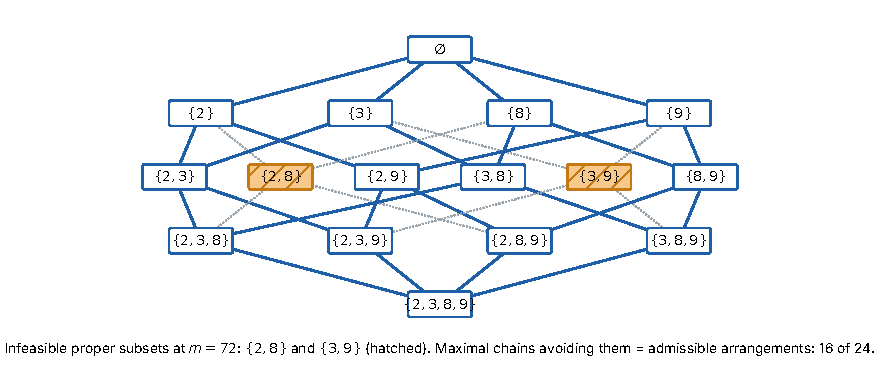
\includegraphics[width=\textwidth]{fig11_feasible_subsets}
\caption{\textbf{Feasible-subset diagram of $\{2,3,8,9\}$ at $m=72$ (exact).} The Boolean lattice of subsets; the two infeasible proper subsets $\{2,8\}$ and $\{3,9\}$ are hatched orange, and the edges at them are dotted grey. The maximal chains $\emptyset\subset\cdots\subset C$ that avoid them are the admissible arrangements: $16$ of the $24$. Theorem illustrated: \cref{cor:P}, \cref{thm:sphere}.}\label{fig:lattice}
\end{figure}

\subsection{The route complexes}
The permutohedron $P_k$ is the convex hull of the points $(\sigma(1),\dots,\sigma(k))\in\mathbb R^k$, $\sigma$ a permutation; it is a simple $(k-1)$-polytope whose boundary is homeomorphic to $S^{k-2}$, and its faces correspond to the ordered set partitions $(B_1|\cdots|B_j)$ of the labels, with dimension $k-j$ and vertex set the arrangements that list $B_1$ first (in any order), then $B_2,\dots$ (see Ziegler~\cite[Example~0.10]{Ziegler1995}). The vertices are the arrangements and the edges are the exchanges of adjacent letters.
\begin{definition}[route complexes]\label{def:routecx}
For a set $\mathcal A$ of arrangements, the \emph{permutohedral route complex} $K_{\mathcal A}$ is the full subcomplex of the face complex of $P_k$ on the vertex set $\mathcal A$: a face is kept iff all its vertices lie in $\mathcal A$. The \emph{cubical route complex} $Q_{\mathcal A}$ is the subcomplex of faces all of whose blocks have size $\le2$ (products of edges): its vertices are the admissible histories, its edges the legal swaps, and its squares and cubes the sets of independent swaps (\cref{lem:indep}). We write $K_m=K_{\mathcal A(m)}$ and $Q_m$. Homology is over $\mathbb F_2$ unless stated. The $1$-skeleton of either complex is the swap graph, so $\beta_0$ counts swap classes. A hexagon (braid relation $xyz\leftrightarrow zyx$) is a $2$-face of $K_m$ iff all six arrangements of the three letters are admissible, and is \emph{never} a cell of $Q_m$.
\end{definition}
\begin{remark}
Faces of $P_k$ containing a given vertex $v$ correspond to subsets of the $k-1$ adjacent position pairs of $v$ (the blocks are the maximal intervals joined by the chosen pairs); this is the simplicity of $P_k$ and is used in \cref{thm:lower}.
\end{remark}

\subsection{Alexander duality}
Write $\mathcal R=\mathfrak S_k\setminus\mathcal A$ for the set of non-admissible arrangements and $\mathcal N(\mathcal R)$ for the simplicial complex on $\mathcal R$ whose simplices are the subsets of $\mathcal R$ contained in a common proper face of $P_k$.
The nerve theorem and Alexander duality used below are in~\cite{Hatcher2002}; the permutohedron is described in~\cite{Ziegler1995}.
\begin{theorem}[duality for route complexes]\label{thm:dual}
Let $\emptyset\ne\mathcal A\ne\mathfrak S_k$. Then $K_{\mathcal A}\subset\partial P_k\cong S^{k-2}$ and, over $\mathbb F_2$, for all $i$
\[
 \dim\tilde H_i(K_{\mathcal A})=\dim\tilde H^{\,k-3-i}\bigl(\mathcal N(\mathcal R)\bigr).
\]
Two vertices of $\mathcal R$ lie in a common proper face iff they share a proper prefix set; hence $\mathcal N(\mathcal R)$ has the connected components of the graph on $\mathcal R$ joined by ``share a proper prefix set''. Consequently $\tilde\beta_{k-2}(K_{\mathcal A})=0$ and $\tilde\beta_{k-3}(K_{\mathcal A})=c(\mathcal R)-1$, where $c(\mathcal R)$ is the number of such components. In particular for $k=3$, $\tilde\beta_1=0$; for $k=4$, $\beta_2=0$ and $\beta_1=c(\mathcal R)-1$; for $k=5$, $\beta_3=0$ and $\beta_2=c(\mathcal R)-1$.
\end{theorem}
\begin{proof}
$K_{\mathcal A}$ is a proper nonempty subcomplex of the sphere $\partial P_k$ (a vertex of $\mathcal R$ lies outside it). A point $x\in\partial P_k$ lies in the relative interior of a unique face $F$, and $x\in K_{\mathcal A}$ iff all vertices of $F$ lie in $\mathcal A$. Hence the complement of $K_{\mathcal A}$ is the union, over $v\in\mathcal R$, of the open stars $\mathrm{st}(v)$ (the union of the relative interiors of the faces containing $v$). Each open star is open in $\partial P_k$ (its complement is the union of the faces not containing $v$) and contractible (it is star-shaped from $v$). For a family $v_1,\dots,v_n$ the intersection $\bigcap\mathrm{st}(v_i)$ is the union of the relative interiors of the faces containing all $v_i$; these are the faces containing the smallest face $\Phi$ containing all $v_i$ (an intersection of faces is a face), so the intersection is $\mathrm{st}(\Phi)$, which is contractible, provided $\Phi$ is a proper face, and it is empty otherwise (there is no proper face containing all $v_i$). By the nerve theorem for open covers~\cite[Cor.~4G.3]{Hatcher2002} the complement of $K_{\mathcal A}$ is homotopy equivalent to the nerve of this cover, which is $\mathcal N(\mathcal R)$. Alexander duality~\cite[Prop.~3.46]{Hatcher2002} applied to the compact, locally contractible, nonempty proper subspace $K_{\mathcal A}$ of $S^{k-2}$ gives $\tilde H_j(S^{k-2}\setminus K_{\mathcal A})\cong\tilde H^{k-3-j}(K_{\mathcal A})$; over a field $\tilde H^q$ and $\tilde H_q$ of a finite complex have equal dimension, which gives the displayed equality after exchanging the roles of the two sides. Two vertices lie in a common proper face iff they lie in a face $(B_1|\cdots|B_j)$ with $j\ge2$, i.e.\ iff they both begin with the proper subset $B_1$, i.e.\ share a proper prefix set. Finally $\tilde H^{-1}$ of a nonempty complex vanishes (this gives $\tilde\beta_{k-2}=0$) and $\tilde\beta^0$ counts components minus one.
\end{proof}
\prov{CW-0359}{T-DUAL}{PROVED}{FULL}
\emph{Check.} The identity $\beta_{k-3}=c(\mathcal R)-1$ (and $\beta_{k-2}=0$) was verified against independent direct homology computations for $1772$ complexes with $k=4,5$ (a sample of contents with labels $\le14$, resp.\ $\le11$, and all sources in the lcm-closure), with no violation (\texttt{results/RESULTS\_II\_part3.json}). \stat{finite-exact} corroboration.

\subsection{Lower sets are contractible}
Fix a total order $\tau$ on the labels. The \emph{weak order} on arrangements is $u\le v$ iff the inversion set of $u$ (pairs ordered differently from $\tau$) is contained in that of $v$; its minimum is the $\tau$-sorted word $b$ and its maximum the reverse. A set $\mathcal A$ is a \emph{lower set} if it is closed under replacing an adjacent inverted pair by the non-inverted one.
\begin{theorem}[lower sets]\label{thm:lower}
If $\mathcal A$ is a nonempty lower set of the weak order, then $K_{\mathcal A}$ is contractible. Consequently, if the feeding digraph of $C$ is acyclic, then $K_m$ is empty or contractible for every source $m$.
\end{theorem}
\begin{proof}
If $\mathcal A=\mathfrak S_k$ then $K_{\mathcal A}$ is the single cell $P_k$; otherwise $b\in\mathcal A$ since $\mathcal A$ is nonempty and a lower set. Induct on $|\mathcal A|$; for $\mathcal A=\{b\}$ the complex is a point. Let $v\ne b$ be maximal in $\mathcal A$. Faces of $P_k$ through $v$ correspond to subsets $J$ of the $k-1$ adjacent position pairs of $v$. If $J$ contains an ascent of $v$ (an adjacent pair in $\tau$-order), the face contains the neighbour of $v$ obtained by exchanging it, which has one more inversion and is not in $\mathcal A$ by maximality. If $J$ consists of descents only, each block of the face is a segment of a decreasing run, so all vertices of the face are obtained from $v$ by sorting inside blocks and are $\le v$, hence in $\mathcal A$. So the faces of $K_{\mathcal A}$ through $v$ correspond to the subsets of $\mathrm{Desc}(v)$, nonempty because $v\ne b$: the link of $v$ in $K_{\mathcal A}$ is a full simplex $L$ (contractible), and the closed star of $v$ is a cone over it. Then $K_{\mathcal A}=K_{\mathcal A\setminus\{v\}}\cup\mathrm{star}(v)$ with $K_{\mathcal A\setminus\{v\}}\cap\mathrm{star}(v)=L$; gluing a cone along its contractible base does not change the homotopy type, so $K_{\mathcal A}\simeq K_{\mathcal A\setminus\{v\}}$, and $\mathcal A\setminus\{v\}$ is again a nonempty lower set. For the consequence: choose $\tau$ so that feeders come first; if $x$ does not feed $y$ and $x$ is placed after $y$ in $\tau$-order... precisely, an inverted adjacent pair $(x,y)$ ($x$ after $y$ in $\tau$) has $x$ not feeding $y$ because all feeding edges go forward in $\tau$; by \cref{lem:NF} replacing it by $(y,x)$ keeps an admissible word admissible. So $\mathcal A(m)$ is a lower set.
\end{proof}
\prov{CW-0360}{T-LOWER}{PROVED}{FULL}
\emph{Check.} For $303$ nonempty route complexes of contents of four distinct labels with acyclic feeding digraph (labels $\le15$, sources among the thresholds), every $K_m$ has Betti vector $(1,0,0,0)$; no violation. \stat{finite-exact} corroboration.

\subsection{Complementary pairs and spheres}
\begin{theorem}[complementary-pair deadlock]\label{thm:sphere}
Let $C=E\sqcup O$ be a partition into nonempty sets and suppose the infeasible proper subsets of $C$ at $m$ are exactly $E$ and $O$. Then $K_m$ has the $\mathbb F_2$-homology of the sphere $S^{k-3}$: $\beta_0=1$ and $\beta_{k-3}=1$ with all other Betti numbers zero (for $k=3$: two points, $\beta_0=2$, the antipodal pair of \cref{thm:T3}).
\end{theorem}
\begin{proof}
The non-admissible arrangements are those having $E$ or $O$ as a prefix set, i.e.\ $\mathcal R=F_{E|O}\sqcup F_{O|E}$, the vertex sets of two facets. A vertex $v$ of the first facet and a vertex $w$ of the second have no common proper prefix set: a proper prefix set of $v$ of size $s\le|E|$ is a subset of $E$ and for $s\ge|E|$ contains $E$, symmetrically for $w$ with $O$; equality of such sets is impossible unless the set is $C$ (the sets would have to lie in both $E$ and $O$, or contain both). Hence $\mathcal N(\mathcal R)$ has exactly two components, each a full simplex (all vertices of a facet lie in a common proper face). So $\tilde H^0(\mathcal N(\mathcal R))$ has rank one and all other reduced groups vanish, and \cref{thm:dual} gives $\tilde\beta_{k-3}=1$ and all other reduced Betti numbers $0$.
\end{proof}
\prov{CW-0361}{T-SPHERE}{PROVED}{FULL}
\begin{remark}[scope]
The homotopy type of $K_m$ is not determined by this argument: it is a statement about $\mathbb F_2$-homology. (That $K_m$ is homotopy equivalent to $S^{k-3}$ would follow if the union of the open stars of the vertices of each facet were an open ball in the sphere, which is plausible but not proved here.) The arithmetic hypothesis (infeasible subsets exactly $E$ and $O$) is a condition on $(C,m)$ that is checked case by case, not a theorem.
\end{remark}
\begin{proposition}[arithmetic realisation; finite-exact]\label{prop:realise}
Let $X$ be a set of labels $n\equiv2,3\pmod6$, $n\ge8$, $C=\{2,3\}\cup X$ and $m=\prod_{x\in X}x$. For all $X\subseteq\{8,9,14,15,20,21\}$ with $1\le|X|\le3$ ($41$ contents) the infeasible proper subsets of $C$ at $m$ are exactly $E=\{x\in C:x\equiv2\bmod 6\}$ and $O=\{x\in C:x\equiv3\bmod6\}$, and the Betti vector of $K_m$ is that of $S^{k-3}$. \stat{finite-exact}.
\end{proposition}
Two instances are the examples that drive the manuscript.
\begin{example}[loop: $\{2,3,8,9\}$ at $72$]\label{ex:loop}
$E=\{2,8\}$, $O=\{3,9\}$, $m=8\cdot9=72$. Of the $24$ arrangements $16$ are admissible, the swap graph is connected, and $K_{72}$ has $f$-vector $(16,20,4)$ (four $2$-faces) and Betti vector $(1,1,0,0)$: a loop of legal swaps that is not filled. The cubical complex $Q_{72}$ has the same $f$-vector and the same Betti vector. The loop is invisible to the connectivity classification (\cref{fig:lattice}, \cref{fig:loop}).
\end{example}
\begin{example}[void: $\{2,3,8,9,14\}$ at $1008$]\label{ex:void}
$E=\{2,8,14\}$, $O=\{3,9\}$, $m=8\cdot9\cdot14=1008$. There are $96$ admissible arrangements out of $120$; $K_{1008}$ has $f$-vector $(96,180,98,12)$ and Betti vector $(1,0,1,0,0)$: a $2$-dimensional void. The cubical complex $Q_{1008}$ has $f$-vector $(96,180,66)$ and Betti vector $(1,19,0,0,0)$: nineteen loops and no void, so the genuine obstruction is seen only after the braid hexagons are filled (\cref{fig:void}).
\end{example}
\begin{figure}[tbp]\centering
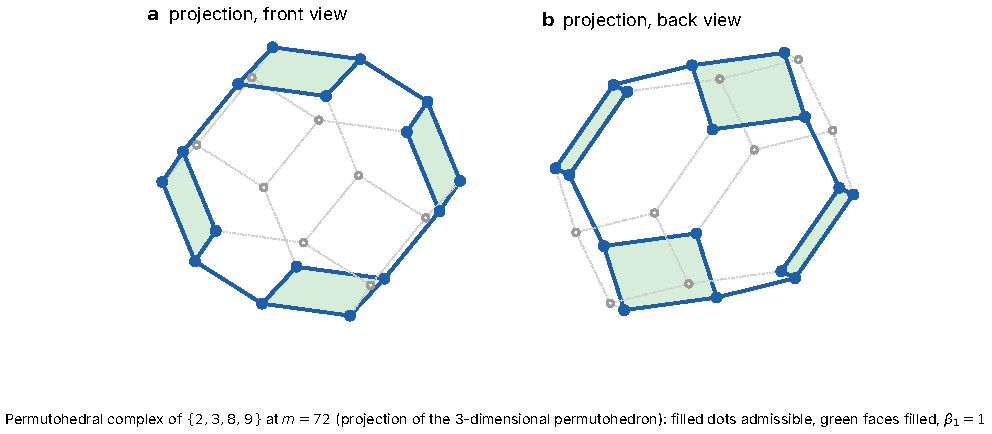
\includegraphics[width=\textwidth]{fig12_four_label_H1}
\caption{\textbf{The permutohedral route complex of $\{2,3,8,9\}$ at $m=72$ (exact; projection of a $3$-dimensional polytope to the plane, front and back views).} Filled blue dots are admissible arrangements, hollow dots are inadmissible; solid blue lines are legal swaps and dotted grey lines are non-legal exchanges; green faces are the four $2$-faces (squares and hexagons) all of whose vertices are admissible. The unfilled cycle of legal swaps is the generator of $H_1=\mathbb F_2$. The picture is a projection; the object is the $3$-dimensional permutohedron's boundary $S^2$. Theorems illustrated: \cref{thm:sphere}, \cref{ex:loop}.}\label{fig:loop}
\end{figure}
\begin{figure}[tbp]\centering
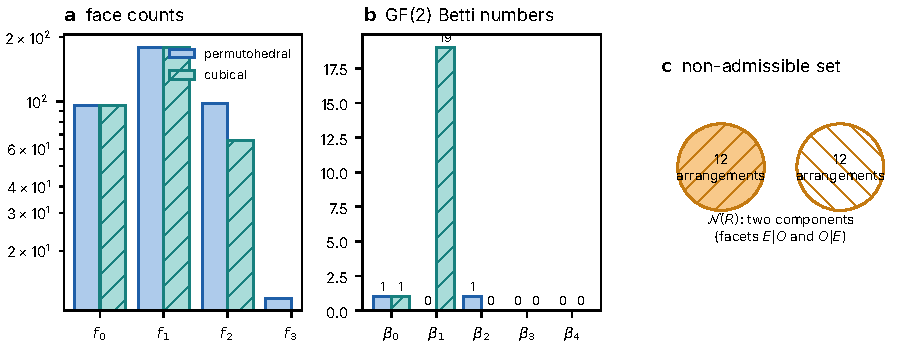
\includegraphics[width=\textwidth]{fig13_five_label_H2}
\caption{\textbf{The void of $\{2,3,8,9,14\}$ at $m=1008$ (exact; incidence data, not a drawing of the $4$-dimensional polytope).} (a) Face counts of the permutohedral complex $K_{1008}$ and of the cubical complex $Q_{1008}$ ($f_0,\dots,f_3$; logarithmic scale). (b) $\mathbb F_2$-Betti numbers: $(1,0,1,0,0)$ for $K_{1008}$ (blue, plain) and $(1,19,0,0,0)$ for $Q_{1008}$ (teal, hatched). (c) The non-admissible set $\mathcal R$ has $24$ arrangements in two components of $\mathcal N(\mathcal R)$ ($12$ and $12$, the facets $E|O$ and $O|E$), whence $\beta_2=2-1=1$ by \cref{thm:dual}. Theorems illustrated: \cref{thm:dual}, \cref{thm:sphere}, \cref{ex:void}.}\label{fig:void}
\end{figure}
\begin{proposition}[cubical versus permutohedral; finite-exact]\label{prop:cubperm}
For the full sets of arrangements ($P(C)\mid m$) of $k=3,4,5$ distinct labels, $K_m$ is a single cell (contractible), while $Q_m$ has Betti vectors $(1,1)$, $(1,7)$, $(1,31)$ respectively, computed here for $C=\{2,3,5\}$, $\{2,3,5,7\}$, $\{2,3,5,7,11\}$ at $m=P(C)$. So a cube-only complex reports loops that are mere braid relations. For $\{2,3,8,9\}$ at $72$ the two complexes agree (\cref{ex:loop}); for $\{2,3,8,9,14\}$ at $1008$ they differ in the way stated in \cref{ex:void}.
\end{proposition}
\prov{CW-0362}{ROUTE\_TOPOLOGY:Cubical-versus-permutohedral}{FINITE-EXACT}{FINITE}

\subsection{Loop family and census}
\begin{proposition}[loop family; finite-exact]\label{prop:loopfam}
For $8\le N<M<40$ with $N,M\equiv2,3\pmod 6$, the content $\{2,3,N,M\}$ has $\beta_1(K_{NM})>0$ (computed here for all such pairs). The programme's records state the converse over $4\le N<M\le60$ (a first Betti number appears at some source only if $N,M\ge8$ and $N,M\equiv2,3\bmod6$); this converse was not re-run here and is \stat{cited}.
\end{proposition}
\begin{proposition}[census; cited]\label{prop:census}
The programme's census over all sources in the lcm-closure records, for $k=3$ (labels $\le30$): $16\,378$ (content, source) pairs, Betti $(1,0,0)$ for $16\,251$ and $(2,0,0)$ for $127$; for $k=4$ (labels $\le18$): $27\,751$ pairs, of which $27\,321$ contractible, $16$ with $(1,1,0,0)$, $405$ with $(2,0,0,0)$, $7$ with $(3,0,0,0)$, $2$ with $(4,0,0,0)$; for $k=5$ (labels $\le11$): $8\,884$ pairs, $8\,617$ contractible, $21$ with $(1,1,0,0,0)$, $235$ with $(2,0,0,0,0)$, $11$ with $(3,0,0,0,0)$. No $\beta_i>0$ for $i\ge2$ occurs outside the void of \cref{ex:void} in these ranges. These are inherited finite computations, \stat{cited}, not re-run here.
\end{proposition}
\prov{CW-0363}{ROUTE\_TOPOLOGY:Census-FINITE-EXACT-contents}{FINITE-EXACT}{FINITE}
\begin{problem}[open: wedge of spheres; realisable types]\label{prob:wedge}
Is $K_m$ always a wedge of spheres (every complex found has the homology of one)? Which families of infeasible subsets occur as the infeasible family of an arithmetic content? Is every sphere $S^j$, $0\le j\le k-3$, realised? Repeated labels need a construction by chains of sub-multisets: \cref{prob:repeated}.
\end{problem}
\prov{CW-0364}{ROUTE\_TOPOLOGY:Statement-of-the-general-conje}{OPEN}{OPEN}
